\documentclass[twoside]{book}

% Packages required by doxygen
\usepackage{fixltx2e}
\usepackage{calc}
\usepackage{doxygen}
\usepackage[export]{adjustbox} % also loads graphicx
\usepackage{graphicx}
\usepackage[utf8]{inputenc}
\usepackage{makeidx}
\usepackage{multicol}
\usepackage{multirow}
\PassOptionsToPackage{warn}{textcomp}
\usepackage{textcomp}
\usepackage[nointegrals]{wasysym}
\usepackage[table]{xcolor}

% Font selection
\usepackage[T1]{fontenc}
\usepackage[scaled=.90]{helvet}
\usepackage{courier}
\usepackage{amssymb}
\usepackage{sectsty}
\renewcommand{\familydefault}{\sfdefault}
\allsectionsfont{%
  \fontseries{bc}\selectfont%
  \color{darkgray}%
}
\renewcommand{\DoxyLabelFont}{%
  \fontseries{bc}\selectfont%
  \color{darkgray}%
}
\newcommand{\+}{\discretionary{\mbox{\scriptsize$\hookleftarrow$}}{}{}}

% Page & text layout
\usepackage{geometry}
\geometry{%
  a4paper,%
  top=2.5cm,%
  bottom=2.5cm,%
  left=2.5cm,%
  right=2.5cm%
}
\tolerance=750
\hfuzz=15pt
\hbadness=750
\setlength{\emergencystretch}{15pt}
\setlength{\parindent}{0cm}
\setlength{\parskip}{3ex plus 2ex minus 2ex}
\makeatletter
\renewcommand{\paragraph}{%
  \@startsection{paragraph}{4}{0ex}{-1.0ex}{1.0ex}{%
    \normalfont\normalsize\bfseries\SS@parafont%
  }%
}
\renewcommand{\subparagraph}{%
  \@startsection{subparagraph}{5}{0ex}{-1.0ex}{1.0ex}{%
    \normalfont\normalsize\bfseries\SS@subparafont%
  }%
}
\makeatother

% Headers & footers
\usepackage{fancyhdr}
\pagestyle{fancyplain}
\fancyhead[LE]{\fancyplain{}{\bfseries\thepage}}
\fancyhead[CE]{\fancyplain{}{}}
\fancyhead[RE]{\fancyplain{}{\bfseries\leftmark}}
\fancyhead[LO]{\fancyplain{}{\bfseries\rightmark}}
\fancyhead[CO]{\fancyplain{}{}}
\fancyhead[RO]{\fancyplain{}{\bfseries\thepage}}
\fancyfoot[LE]{\fancyplain{}{}}
\fancyfoot[CE]{\fancyplain{}{}}
\fancyfoot[RE]{\fancyplain{}{\bfseries\scriptsize Generated by Doxygen }}
\fancyfoot[LO]{\fancyplain{}{\bfseries\scriptsize Generated by Doxygen }}
\fancyfoot[CO]{\fancyplain{}{}}
\fancyfoot[RO]{\fancyplain{}{}}
\renewcommand{\footrulewidth}{0.4pt}
\renewcommand{\chaptermark}[1]{%
  \markboth{#1}{}%
}
\renewcommand{\sectionmark}[1]{%
  \markright{\thesection\ #1}%
}

% Indices & bibliography
\usepackage{natbib}
\usepackage[titles]{tocloft}
\setcounter{tocdepth}{3}
\setcounter{secnumdepth}{5}
\makeindex

% Hyperlinks (required, but should be loaded last)
\usepackage{ifpdf}
\ifpdf
  \usepackage[pdftex,pagebackref=true]{hyperref}
\else
  \usepackage[ps2pdf,pagebackref=true]{hyperref}
\fi
\hypersetup{%
  colorlinks=true,%
  linkcolor=blue,%
  citecolor=blue,%
  unicode%
}

% Custom commands
\newcommand{\clearemptydoublepage}{%
  \newpage{\pagestyle{empty}\cleardoublepage}%
}

\usepackage{caption}
\captionsetup{labelsep=space,justification=centering,font={bf},singlelinecheck=off,skip=4pt,position=top}

%===== C O N T E N T S =====

\begin{document}

% Titlepage & ToC
\hypersetup{pageanchor=false,
             bookmarksnumbered=true,
             pdfencoding=unicode
            }
\pagenumbering{roman}
\begin{titlepage}
\vspace*{7cm}
\begin{center}%
{\Large bounswe2016group12 Assignment 6 Ezgi }\\
\vspace*{1cm}
{\large Generated by Doxygen 1.8.11}\\
\end{center}
\end{titlepage}
\clearemptydoublepage
\tableofcontents
\clearemptydoublepage
\pagenumbering{arabic}
\hypersetup{pageanchor=true}

%--- Begin generated contents ---
\chapter{Namespace Index}
\section{Packages}
Here are the packages with brief descriptions (if available)\+:\begin{DoxyCompactList}
\item\contentsline{section}{\hyperlink{namespace_meanco_app_1_1functions_1_1relation}{Meanco\+App.\+functions.\+relation} }{\pageref{namespace_meanco_app_1_1functions_1_1relation}}{}
\item\contentsline{section}{\hyperlink{namespace_meanco_app_1_1functions_1_1search}{Meanco\+App.\+functions.\+search} }{\pageref{namespace_meanco_app_1_1functions_1_1search}}{}
\item\contentsline{section}{\hyperlink{namespace_meanco_app_1_1models_1_1comment}{Meanco\+App.\+models.\+comment} }{\pageref{namespace_meanco_app_1_1models_1_1comment}}{}
\item\contentsline{section}{\hyperlink{namespace_meanco_app_1_1models_1_1profile}{Meanco\+App.\+models.\+profile} }{\pageref{namespace_meanco_app_1_1models_1_1profile}}{}
\item\contentsline{section}{\hyperlink{namespace_meanco_app_1_1models_1_1relation}{Meanco\+App.\+models.\+relation} }{\pageref{namespace_meanco_app_1_1models_1_1relation}}{}
\item\contentsline{section}{\hyperlink{namespace_meanco_app_1_1models_1_1tag}{Meanco\+App.\+models.\+tag} }{\pageref{namespace_meanco_app_1_1models_1_1tag}}{}
\item\contentsline{section}{\hyperlink{namespace_meanco_app_1_1models_1_1topic}{Meanco\+App.\+models.\+topic} }{\pageref{namespace_meanco_app_1_1models_1_1topic}}{}
\item\contentsline{section}{\hyperlink{namespace_meanco_app_1_1serializers}{Meanco\+App.\+serializers} }{\pageref{namespace_meanco_app_1_1serializers}}{}
\item\contentsline{section}{\hyperlink{namespace_meanco_app_1_1tests}{Meanco\+App.\+tests} }{\pageref{namespace_meanco_app_1_1tests}}{}
\item\contentsline{section}{\hyperlink{namespace_meanco_app_1_1views_1_1_api_authentication}{Meanco\+App.\+views.\+Api\+Authentication} }{\pageref{namespace_meanco_app_1_1views_1_1_api_authentication}}{}
\item\contentsline{section}{\hyperlink{namespace_meanco_app_1_1views_1_1_api_comment}{Meanco\+App.\+views.\+Api\+Comment} }{\pageref{namespace_meanco_app_1_1views_1_1_api_comment}}{}
\item\contentsline{section}{\hyperlink{namespace_meanco_app_1_1views_1_1_api_relation}{Meanco\+App.\+views.\+Api\+Relation} }{\pageref{namespace_meanco_app_1_1views_1_1_api_relation}}{}
\item\contentsline{section}{\hyperlink{namespace_meanco_app_1_1views_1_1_api_tag}{Meanco\+App.\+views.\+Api\+Tag} }{\pageref{namespace_meanco_app_1_1views_1_1_api_tag}}{}
\item\contentsline{section}{\hyperlink{namespace_meanco_app_1_1views_1_1_api_topic}{Meanco\+App.\+views.\+Api\+Topic} }{\pageref{namespace_meanco_app_1_1views_1_1_api_topic}}{}
\item\contentsline{section}{\hyperlink{namespace_meanco_app_1_1views_1_1_comment}{Meanco\+App.\+views.\+Comment} }{\pageref{namespace_meanco_app_1_1views_1_1_comment}}{}
\item\contentsline{section}{\hyperlink{namespace_meanco_app_1_1views_1_1forms}{Meanco\+App.\+views.\+forms} }{\pageref{namespace_meanco_app_1_1views_1_1forms}}{}
\item\contentsline{section}{\hyperlink{namespace_meanco_app_1_1views_1_1_home}{Meanco\+App.\+views.\+Home} }{\pageref{namespace_meanco_app_1_1views_1_1_home}}{}
\item\contentsline{section}{\hyperlink{namespace_meanco_app_1_1views_1_1_profile}{Meanco\+App.\+views.\+Profile} }{\pageref{namespace_meanco_app_1_1views_1_1_profile}}{}
\item\contentsline{section}{\hyperlink{namespace_meanco_app_1_1views_1_1_relation}{Meanco\+App.\+views.\+Relation} }{\pageref{namespace_meanco_app_1_1views_1_1_relation}}{}
\item\contentsline{section}{\hyperlink{namespace_meanco_app_1_1views_1_1_search_list}{Meanco\+App.\+views.\+Search\+List} }{\pageref{namespace_meanco_app_1_1views_1_1_search_list}}{}
\end{DoxyCompactList}

\chapter{Hierarchical Index}
\section{Class Hierarchy}
This inheritance list is sorted roughly, but not completely, alphabetically\+:\begin{DoxyCompactList}
\item Http\+Servlet\begin{DoxyCompactList}
\item \contentsline{section}{com.\+ahmet.\+My\+Servlet}{\pageref{classcom_1_1ahmet_1_1_my_servlet}}{}
\end{DoxyCompactList}
\end{DoxyCompactList}

\chapter{Class Index}
\section{Class List}
Here are the classes, structs, unions and interfaces with brief descriptions\+:\begin{DoxyCompactList}
\item\contentsline{section}{\hyperlink{classmain_1_1java_1_1com_1_1ezgi_1_1_ezgis_servlet}{main.\+java.\+com.\+ezgi.\+Ezgis\+Servlet} }{\pageref{classmain_1_1java_1_1com_1_1ezgi_1_1_ezgis_servlet}}{}
\item\contentsline{section}{\hyperlink{classmain_1_1java_1_1com_1_1ezgi_1_1_my_x_m_l_parser}{main.\+java.\+com.\+ezgi.\+My\+X\+M\+L\+Parser} }{\pageref{classmain_1_1java_1_1com_1_1ezgi_1_1_my_x_m_l_parser}}{}
\end{DoxyCompactList}

\chapter{File Index}
\section{File List}
Here is a list of all files with brief descriptions\+:\begin{DoxyCompactList}
\item\contentsline{section}{src/main/java/com/ezgi/\hyperlink{_ezgis_servlet_8java}{Ezgis\+Servlet.\+java} }{\pageref{_ezgis_servlet_8java}}{}
\item\contentsline{section}{src/main/java/com/ezgi/\hyperlink{_my_x_m_l_parser_8java}{My\+X\+M\+L\+Parser.\+java} }{\pageref{_my_x_m_l_parser_8java}}{}
\end{DoxyCompactList}

\chapter{Namespace Documentation}
\hypertarget{namespacemain}{}\section{Package main}
\label{namespacemain}\index{main@{main}}
\subsection*{Packages}
\begin{DoxyCompactItemize}
\item 
package \hyperlink{namespacemain_1_1java}{java}
\end{DoxyCompactItemize}

\hypertarget{namespacemain_1_1java}{}\section{Package main.\+java}
\label{namespacemain_1_1java}\index{main.\+java@{main.\+java}}
\subsection*{Packages}
\begin{DoxyCompactItemize}
\item 
package \hyperlink{namespacemain_1_1java_1_1com}{com}
\end{DoxyCompactItemize}

\hypertarget{namespacemain_1_1java_1_1com}{}\section{Package main.\+java.\+com}
\label{namespacemain_1_1java_1_1com}\index{main.\+java.\+com@{main.\+java.\+com}}
\subsection*{Packages}
\begin{DoxyCompactItemize}
\item 
package \hyperlink{namespacemain_1_1java_1_1com_1_1ezgi}{ezgi}
\end{DoxyCompactItemize}

\hypertarget{namespacemain_1_1java_1_1com_1_1ezgi}{}\section{Package main.\+java.\+com.\+ezgi}
\label{namespacemain_1_1java_1_1com_1_1ezgi}\index{main.\+java.\+com.\+ezgi@{main.\+java.\+com.\+ezgi}}
\subsection*{Classes}
\begin{DoxyCompactItemize}
\item 
class \hyperlink{classmain_1_1java_1_1com_1_1ezgi_1_1_ezgis_servlet}{Ezgis\+Servlet}
\item 
class \hyperlink{classmain_1_1java_1_1com_1_1ezgi_1_1_my_x_m_l_parser}{My\+X\+M\+L\+Parser}
\end{DoxyCompactItemize}

\chapter{Class Documentation}
\hypertarget{classmain_1_1java_1_1com_1_1ezgi_1_1_ezgis_servlet}{}\section{main.\+java.\+com.\+ezgi.\+Ezgis\+Servlet Class Reference}
\label{classmain_1_1java_1_1com_1_1ezgi_1_1_ezgis_servlet}\index{main.\+java.\+com.\+ezgi.\+Ezgis\+Servlet@{main.\+java.\+com.\+ezgi.\+Ezgis\+Servlet}}
Inheritance diagram for main.\+java.\+com.\+ezgi.\+Ezgis\+Servlet\+:\begin{figure}[H]
\begin{center}
\leavevmode
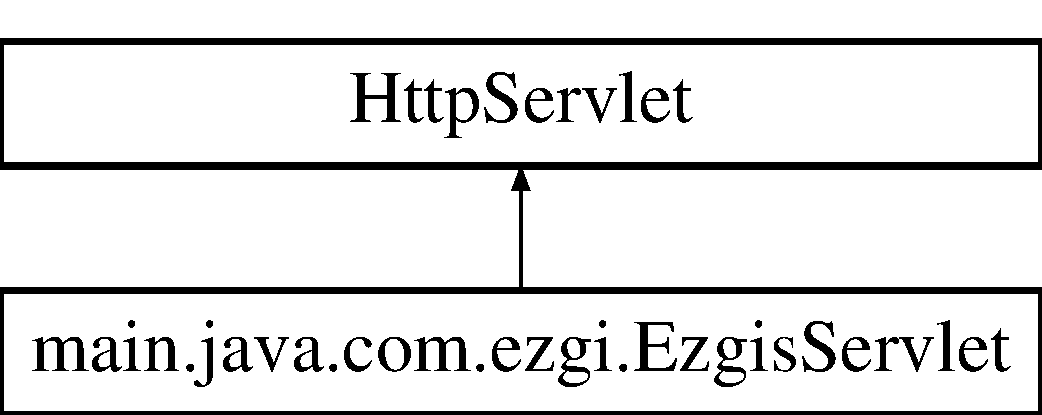
\includegraphics[height=2.000000cm]{classmain_1_1java_1_1com_1_1ezgi_1_1_ezgis_servlet}
\end{center}
\end{figure}
\subsection*{Protected Member Functions}
\begin{DoxyCompactItemize}
\item 
void \hyperlink{classmain_1_1java_1_1com_1_1ezgi_1_1_ezgis_servlet_a2e3fb2c681dba396ae8f841367d49bab}{do\+Post} (Http\+Servlet\+Request request, Http\+Servlet\+Response response)  throws Servlet\+Exception, I\+O\+Exception 
\item 
void \hyperlink{classmain_1_1java_1_1com_1_1ezgi_1_1_ezgis_servlet_aeaebad3b7b8373e1d43027b47c0b4cc5}{do\+Get} (Http\+Servlet\+Request request, Http\+Servlet\+Response response)  throws Servlet\+Exception, I\+O\+Exception 
\end{DoxyCompactItemize}


\subsection{Detailed Description}
Created by Ezgi on 5/6/2016. 

\subsection{Member Function Documentation}
\index{main\+::java\+::com\+::ezgi\+::\+Ezgis\+Servlet@{main\+::java\+::com\+::ezgi\+::\+Ezgis\+Servlet}!do\+Get@{do\+Get}}
\index{do\+Get@{do\+Get}!main\+::java\+::com\+::ezgi\+::\+Ezgis\+Servlet@{main\+::java\+::com\+::ezgi\+::\+Ezgis\+Servlet}}
\subsubsection[{\texorpdfstring{do\+Get(\+Http\+Servlet\+Request request, Http\+Servlet\+Response response)}{doGet(HttpServletRequest request, HttpServletResponse response)}}]{\setlength{\rightskip}{0pt plus 5cm}void main.\+java.\+com.\+ezgi.\+Ezgis\+Servlet.\+do\+Get (
\begin{DoxyParamCaption}
\item[{Http\+Servlet\+Request}]{request, }
\item[{Http\+Servlet\+Response}]{response}
\end{DoxyParamCaption}
) throws Servlet\+Exception, I\+O\+Exception\hspace{0.3cm}{\ttfamily [protected]}}\hypertarget{classmain_1_1java_1_1com_1_1ezgi_1_1_ezgis_servlet_aeaebad3b7b8373e1d43027b47c0b4cc5}{}\label{classmain_1_1java_1_1com_1_1ezgi_1_1_ezgis_servlet_aeaebad3b7b8373e1d43027b47c0b4cc5}
\index{main\+::java\+::com\+::ezgi\+::\+Ezgis\+Servlet@{main\+::java\+::com\+::ezgi\+::\+Ezgis\+Servlet}!do\+Post@{do\+Post}}
\index{do\+Post@{do\+Post}!main\+::java\+::com\+::ezgi\+::\+Ezgis\+Servlet@{main\+::java\+::com\+::ezgi\+::\+Ezgis\+Servlet}}
\subsubsection[{\texorpdfstring{do\+Post(\+Http\+Servlet\+Request request, Http\+Servlet\+Response response)}{doPost(HttpServletRequest request, HttpServletResponse response)}}]{\setlength{\rightskip}{0pt plus 5cm}void main.\+java.\+com.\+ezgi.\+Ezgis\+Servlet.\+do\+Post (
\begin{DoxyParamCaption}
\item[{Http\+Servlet\+Request}]{request, }
\item[{Http\+Servlet\+Response}]{response}
\end{DoxyParamCaption}
) throws Servlet\+Exception, I\+O\+Exception\hspace{0.3cm}{\ttfamily [protected]}}\hypertarget{classmain_1_1java_1_1com_1_1ezgi_1_1_ezgis_servlet_a2e3fb2c681dba396ae8f841367d49bab}{}\label{classmain_1_1java_1_1com_1_1ezgi_1_1_ezgis_servlet_a2e3fb2c681dba396ae8f841367d49bab}


The documentation for this class was generated from the following file\+:\begin{DoxyCompactItemize}
\item 
src/main/java/com/ezgi/\hyperlink{_ezgis_servlet_8java}{Ezgis\+Servlet.\+java}\end{DoxyCompactItemize}

\hypertarget{classmain_1_1java_1_1com_1_1ezgi_1_1_my_x_m_l_parser}{}\section{main.\+java.\+com.\+ezgi.\+My\+X\+M\+L\+Parser Class Reference}
\label{classmain_1_1java_1_1com_1_1ezgi_1_1_my_x_m_l_parser}\index{main.\+java.\+com.\+ezgi.\+My\+X\+M\+L\+Parser@{main.\+java.\+com.\+ezgi.\+My\+X\+M\+L\+Parser}}
\subsection*{Public Member Functions}
\begin{DoxyCompactItemize}
\item 
\hyperlink{classmain_1_1java_1_1com_1_1ezgi_1_1_my_x_m_l_parser_a9a523df969a1b850073d257b0b7c248e}{My\+X\+M\+L\+Parser} (String query)
\item 
String \hyperlink{classmain_1_1java_1_1com_1_1ezgi_1_1_my_x_m_l_parser_a8a91548324095ae97b5f48deb999af89}{read\+X\+ML} (String url)  throws I\+O\+Exception 
\item 
void \hyperlink{classmain_1_1java_1_1com_1_1ezgi_1_1_my_x_m_l_parser_a3472904de01c66bd431d08b11b99242b}{get\+Data} ()  throws I\+O\+Exception, S\+A\+X\+Exception, Parser\+Configuration\+Exception 
\end{DoxyCompactItemize}


\subsection{Constructor \& Destructor Documentation}
\index{main\+::java\+::com\+::ezgi\+::\+My\+X\+M\+L\+Parser@{main\+::java\+::com\+::ezgi\+::\+My\+X\+M\+L\+Parser}!My\+X\+M\+L\+Parser@{My\+X\+M\+L\+Parser}}
\index{My\+X\+M\+L\+Parser@{My\+X\+M\+L\+Parser}!main\+::java\+::com\+::ezgi\+::\+My\+X\+M\+L\+Parser@{main\+::java\+::com\+::ezgi\+::\+My\+X\+M\+L\+Parser}}
\subsubsection[{\texorpdfstring{My\+X\+M\+L\+Parser(\+String query)}{MyXMLParser(String query)}}]{\setlength{\rightskip}{0pt plus 5cm}main.\+java.\+com.\+ezgi.\+My\+X\+M\+L\+Parser.\+My\+X\+M\+L\+Parser (
\begin{DoxyParamCaption}
\item[{String}]{query}
\end{DoxyParamCaption}
)}\hypertarget{classmain_1_1java_1_1com_1_1ezgi_1_1_my_x_m_l_parser_a9a523df969a1b850073d257b0b7c248e}{}\label{classmain_1_1java_1_1com_1_1ezgi_1_1_my_x_m_l_parser_a9a523df969a1b850073d257b0b7c248e}


\subsection{Member Function Documentation}
\index{main\+::java\+::com\+::ezgi\+::\+My\+X\+M\+L\+Parser@{main\+::java\+::com\+::ezgi\+::\+My\+X\+M\+L\+Parser}!get\+Data@{get\+Data}}
\index{get\+Data@{get\+Data}!main\+::java\+::com\+::ezgi\+::\+My\+X\+M\+L\+Parser@{main\+::java\+::com\+::ezgi\+::\+My\+X\+M\+L\+Parser}}
\subsubsection[{\texorpdfstring{get\+Data()}{getData()}}]{\setlength{\rightskip}{0pt plus 5cm}void main.\+java.\+com.\+ezgi.\+My\+X\+M\+L\+Parser.\+get\+Data (
\begin{DoxyParamCaption}
{}
\end{DoxyParamCaption}
) throws I\+O\+Exception, S\+A\+X\+Exception, Parser\+Configuration\+Exception}\hypertarget{classmain_1_1java_1_1com_1_1ezgi_1_1_my_x_m_l_parser_a3472904de01c66bd431d08b11b99242b}{}\label{classmain_1_1java_1_1com_1_1ezgi_1_1_my_x_m_l_parser_a3472904de01c66bd431d08b11b99242b}
\index{main\+::java\+::com\+::ezgi\+::\+My\+X\+M\+L\+Parser@{main\+::java\+::com\+::ezgi\+::\+My\+X\+M\+L\+Parser}!read\+X\+ML@{read\+X\+ML}}
\index{read\+X\+ML@{read\+X\+ML}!main\+::java\+::com\+::ezgi\+::\+My\+X\+M\+L\+Parser@{main\+::java\+::com\+::ezgi\+::\+My\+X\+M\+L\+Parser}}
\subsubsection[{\texorpdfstring{read\+X\+M\+L(\+String url)}{readXML(String url)}}]{\setlength{\rightskip}{0pt plus 5cm}String main.\+java.\+com.\+ezgi.\+My\+X\+M\+L\+Parser.\+read\+X\+ML (
\begin{DoxyParamCaption}
\item[{String}]{url}
\end{DoxyParamCaption}
) throws I\+O\+Exception}\hypertarget{classmain_1_1java_1_1com_1_1ezgi_1_1_my_x_m_l_parser_a8a91548324095ae97b5f48deb999af89}{}\label{classmain_1_1java_1_1com_1_1ezgi_1_1_my_x_m_l_parser_a8a91548324095ae97b5f48deb999af89}


The documentation for this class was generated from the following file\+:\begin{DoxyCompactItemize}
\item 
src/main/java/com/ezgi/\hyperlink{_my_x_m_l_parser_8java}{My\+X\+M\+L\+Parser.\+java}\end{DoxyCompactItemize}

\chapter{File Documentation}
\hypertarget{_ezgis_servlet_8java}{}\section{src/main/java/com/ezgi/\+Ezgis\+Servlet.java File Reference}
\label{_ezgis_servlet_8java}\index{src/main/java/com/ezgi/\+Ezgis\+Servlet.\+java@{src/main/java/com/ezgi/\+Ezgis\+Servlet.\+java}}
\subsection*{Classes}
\begin{DoxyCompactItemize}
\item 
class \hyperlink{classmain_1_1java_1_1com_1_1ezgi_1_1_ezgis_servlet}{main.\+java.\+com.\+ezgi.\+Ezgis\+Servlet}
\end{DoxyCompactItemize}
\subsection*{Packages}
\begin{DoxyCompactItemize}
\item 
package \hyperlink{namespacemain_1_1java_1_1com_1_1ezgi}{main.\+java.\+com.\+ezgi}
\end{DoxyCompactItemize}

\hypertarget{_my_x_m_l_parser_8java}{}\section{src/main/java/com/ezgi/\+My\+X\+M\+L\+Parser.java File Reference}
\label{_my_x_m_l_parser_8java}\index{src/main/java/com/ezgi/\+My\+X\+M\+L\+Parser.\+java@{src/main/java/com/ezgi/\+My\+X\+M\+L\+Parser.\+java}}
\subsection*{Classes}
\begin{DoxyCompactItemize}
\item 
class \hyperlink{classmain_1_1java_1_1com_1_1ezgi_1_1_my_x_m_l_parser}{main.\+java.\+com.\+ezgi.\+My\+X\+M\+L\+Parser}
\end{DoxyCompactItemize}
\subsection*{Packages}
\begin{DoxyCompactItemize}
\item 
package \hyperlink{namespacemain_1_1java_1_1com_1_1ezgi}{main.\+java.\+com.\+ezgi}
\end{DoxyCompactItemize}

%--- End generated contents ---

% Index
\backmatter
\newpage
\phantomsection
\clearemptydoublepage
\addcontentsline{toc}{chapter}{Index}
\printindex

\end{document}
